% \textbf{\underline{OZ 5 - Magnetische inductie en de wet van Faraday - Oefening 5:}}
% \vspace{0.5cm}

% Een homogeen magnetisch veld wordt aangelegd in een cirkel met straal $ R $, zoals aangegeven op Figuur 5.5. Het veld verandert in de tijd volgens $ B = (2,00t^3 - 4,00t^2 + 0,800) $ T met $ t $ de tijds in seconden. Zij $ r_2 = 2R = 5,00 $ cm.

% \begin{enumerate}[(a)]
%     \item Bereken de grootte en richting van de kracht die inwerkt op een elektron dat zich in punt $ P_2 $ bevindt als $ t = 2,00 $ s.
%     \item Op welk tijdstip is deze kracht gelijk aan nul?
% \end{enumerate}

% \begin{figure}[H]
%     \centering
%     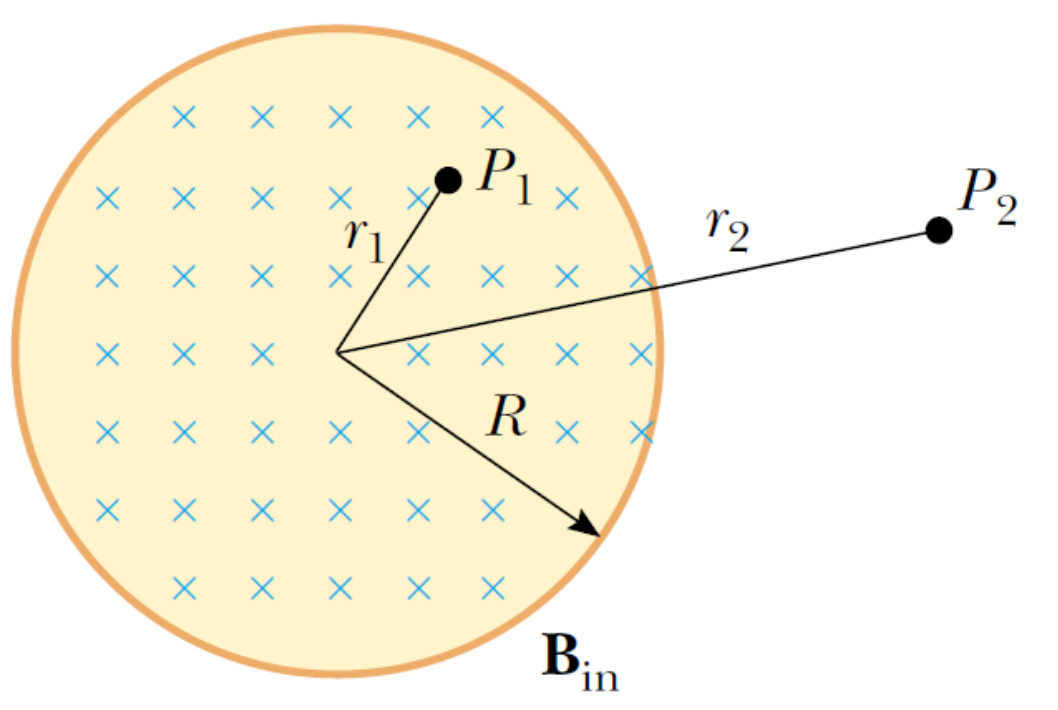
\includegraphics[width=4cm]{oz05/resources/oef-5-opgave.png}
    
%     \textbf{Figuur 5.5}
% \end{figure}

% \begin{description}[labelwidth=1.5cm, leftmargin=!]
%     \item[Geg. :]   $ R = 2,5 $ cm; $ B = \left( 2,00t^3 - 4,00t^2 + 0,800 \right) $ T; $ r_2 = 5,00 $ cm;
% \end{description}

% \begin{enumerate}[(a)]
%     \item 
%         \begin{description}[labelwidth=1.5cm, leftmargin=!]
%             \item[Gevr. :]  $ F $ op $ P_2 $ wanneer $ t = 2,00 $ s;
%             \item[Opl. :]   $ \Phi_B = \int \vec{B} \cdot d\vec{A} 
%                             = B \cdot \pi \cdot R^2 
%                             = \left( 2,00t^3 - 4,00t^2 + 0,800 \right) \cdot \pi \cdot (2,5 \cdot 10^{-2})^2 $ 
                            
%                             \hspace{0.48cm} $ 
%                             = \pi (0,00125t^3 - 0,0025t^2 + 0,00078125) $ Wb
                            
%                             \vspace{0.5cm}
                            
%                             $ \dfrac{d\Phi_B}{dt} = (3 \cdot 0,00125 t^2 - 2 \cdot 0,0025 t)\pi $ Wb/s $ = (0,00375t^2 - 0,005t)\pi $ Wb/s
                            
%                             \vspace{0.5cm}
                            
%                             $ \oint{\vec{E} \cdot d\vec{s}} = -\dfrac{d\Phi_B}{dt} $
                            
%                             \hspace{-0.57cm} $ \Rightarrow
%                             E \cdot 2\pi \cdot r_2 = -\dfrac{d\Phi_B}{dt} $
                            
%                             \hspace{-0.57cm} $ \Leftrightarrow
%                             E = -\dfrac{1}{2\pi \cdot r_2} \cdot \dfrac{d\Phi_B}{dt} 
%                             = -\dfrac{1}{2\pi \cdot (5,00 \cdot 10^{-2})} \cdot (0,00375t^2 - 0,005t)\pi $
                            
%                             \hspace{0.275cm} $
%                             = -(0,0375t^2 - 0,05t)\ $ V/m
                            
%                             \vspace{0.5cm}
                            
%                             $ \vec{F} = q\vec{E} + q\vec{v} \times \vec{B} = -1,60 \cdot 10^{-19} \cdot -(0,0375t^2 - 0,05t) + 0 $
                            
%                             \hspace{-0.57cm} $ \Rightarrow 
%                             F = 1,60 \cdot 10^{-19} \cdot (0,0375\cdot (2,00)^2 - 0,05 \cdot 2,00) = 8 \cdot 10^{-21} $ N $ = 8 $ zN
%         \end{description}
%     \item
%         \begin{description}[labelwidth=1.5cm, leftmargin=!]
%             \item[Gevr. :]  $ t $ op $ P_2 $ wanneer $ F = 0 $ s;
%             \item[Opl. :]   $ F = 1,60 \cdot 10^{-19} \cdot (0,0375 t^2 - 0,05t) $
                            
%                             \hspace{-0.57cm} $ \Leftrightarrow
%                             0 = 1,60 \cdot 10^{-19} \cdot (0,0375 t^2 - 0,05t) $
                            
%                             \hspace{-0.57cm} $ \Leftrightarrow
%                             0 = 0,0375 t^2 - 0,05t $
                            
%                             \hspace{-0.57cm} $ \Leftrightarrow
%                             0 = t(0,0375 t - 0,05) $
                            
%                             \hspace{-0.57cm} $ \Rightarrow
%                             t = 0 $ s \hspace{0.5cm} OF \hspace{0.5cm} $ 0,0375 t - 0,05 = 0 $
                            
%                             \hspace{2.45cm} $ \Leftrightarrow 
%                             t = 1,33 $ s
            
%         \end{description}
% \end{enumerate}

% \vspace{1cm}